\section{Разрезы. Лемма о потоках и разрезах. Следствие.}

\begin{note}
    Рассмотрим двухполюсную сеть $ G = (V,E) $ с источником $ s $, стоком $ t $ и заданной функцией пропускных способностей $ c: E \rightarrow \R_+ $.
\end{note}

\begin{definition}[Разрез]
    Пусть $ W \subset V, \ \widetilde{W} = V \setminus W $. \emph{Разрезом} $ (W, \widetilde{W}) $ в сети $ G $ называется множество всех дуг вида $ e = uv $, где $ u \in W, \ v \in \widetilde{W} $.
\end{definition}

\begin{note}
    Говорят, что разрез разделяет вершины $ s $ и $ t $, если $ s \in W, \ t \in \widetilde{W} $.
\end{note}

\begin{definition}[Пропускная способность]
    \emph{Пропускной способностью} разреза $ (W, \widetilde{W}) $ называется число
    \[
        c(W,\widetilde{W})= \sum_{e \in (W,\widetilde{W})}c(e).
    \]
\end{definition}

\begin{definition}[Минимальный разрез]
    \emph{Минимальным разрезом}, разделяющим $ s $ и $ t $, называется разрез с минимальной пропускной способностью среди всех таких разрезов.
\end{definition}

\begin{definition}[Поток через разрез]
    Если $ f: E \rightarrow \R_+ $ -- поток из $ s $ в $ t $, то потоком через разрез $ (W,\widetilde{W}) $ называется число
    \[
        f(W,\widetilde{W}) = \sum_{e\in(W,\widetilde{W})}f(e).
    \]
\end{definition}

\begin{lemma}[О потоках и разрезах]
    Для любого потока $ f $ из $ s $ в $ t $ и произольного разреза $ (W,\widetilde{W}) $, разделяющего $ s $ и $ t $, имеет место равенство
    \[
        b(f) = f(W,\widetilde{W}) - f(\widetilde{W},W).
    \]
\end{lemma}

\begin{proof}
    Суммируем уравнение баланса
    \[
        \sum_{v\in A(u)}f(uv) - \sum_{v\in B(u)}f(vu) = \left\{\begin{array}{ll}
            b,  & \text{если }u = s            \\
            0,  & \text{если }u \notin \{s,t\} \\
            -b, & \text{если }u = t
        \end{array}\right.
    \]
    по всем вершинам $ u \in W $. В этой сумме каждая дуга вида $ pq $, где $ p \in W, \ q \in W $ встречается дважды: один раз со знаком «$+$» в $ \sum_{v \in A(p)}f(pv) $ и один раз со знаком «$-$» в $ -\sum_{v \in B(q)}f(vq) $, то есть
    \[
        f(pq) - f(pq) = 0.
    \]

    Каждое слагаемое $ f(pq) $, в котором $ p \in W, \ q \in \widetilde{W} $ встречается только один раз со знаком «$+$» в $ \sum_{v \in A(p)}f(pv) $.

    А каждое слагаемое $ f(pq) $, в котором $ p \in \widetilde{W}, \ q \in W $ встречается один раз со знаком «$-$» в $ -\sum_{v \in B(q)}f(vq) $.

    Суммирование левых частей условия баланса:
    \[
        f(W,\widetilde{W}) - f(\widetilde{W},W).
    \]

    Суммирование правых частей в условии баланса по всем вершинам $ u \in W $ даст $ b = b(f) $, так как $ s \in W, \ t \notin W $.
\end{proof}

\begin{corollary}[О потоках и разрезах]
    В любой сети величина любого потока из $ s $ в $ t $ не превосходит пропускной способности любого разреза, разделяющего $ s $ и $ t $.
\end{corollary}

\begin{proof}
    Из леммы о потоках и разрезах с учетом условия допустимости
    \[
        0 \leqslant f(e) \leqslant c(e) \quad \forall e \in E \implies
    \]
    \begin{multline*}
        \implies b(f) = f(W,\widetilde{W}) - f(\underbrace{\widetilde{W}}_{\geqslant 0},W) \leqslant \\
        \leqslant f(W,\widetilde{W}) = \sum_{e \in (W,\widetilde{W})}f(e) \leqslant \\
        \leqslant \sum_{e \in (W,\widetilde{W})}c(e) = c(W,\widetilde{W}).
    \end{multline*}
\end{proof}

\section{Теорема Форда-Фалкерсона.}

\begin{theorem}[Форд-Фалкерсон]
    В любой конечной сети $ G = (V,E) $ величина максимального потока из $ s $ в $ t $ равна пропускной способности минимального разреза, разделяющего $ s $ и $ t $.
\end{theorem}

\begin{proof}
    Пусть $ f^* $ -- максимальный поток из $ s $ в $ t $ в сети $ G = (V,E) $. Построим разрез $ (W,\widetilde{W}) $, разделяющий $ s $ и $ t $:
    \[
        c(W,\widetilde{W}) = b(f^*).
    \]

    \begin{note}[Алгоритм построения минимального разреза]
        Формируем множество $ \widetilde{W} $:
        \begin{enumerate}
            \item $ s \rightarrow W $.
            \item Если $ u \in W $ и $ f^*(uv) < c(uv) $, то $ v \rightarrow W $.
            \item Если $ u \in W $ и $ f^*(uv) > 0 $, то $ v \rightarrow W $.
        \end{enumerate}

        Повторяем пункты $ 2.-3. $ до тех пор, пока это возможно.
    \end{note}

    Заметим, что по окончании алгоритма вершина $ t \notin W $, то есть $ t \in \widetilde{W} = V \setminus W $. Если бы $ t $ попало в $ W $, то в сети $ G $ нашелся бы увеличивающий путь $ P $ для потока $ f^* $, а это не возможно, так как $ f^* $ -- макимальный.

    Мы построили разрез, разделяющий $ s $ и $ t $. По построению:
    \[
        f^*(W,\widetilde{W}) = c(W,\widetilde{W}), \quad f^*(\widetilde{W},W) = 0.
    \]

    По лемме о потоках и разрезах,
    \[
        b(f^*) = \equalto{f^*(W,\widetilde{W})}{c(W,\widetilde{W})} - \equalto{f^*(\widetilde{W},W)}{0} = c(W,\widetilde{W}).
    \]

    По следствию о потоках и разрезах, для любого разреза $ (U,\widetilde{U}) $, разделяющего $ s $ и $ t $,
    \[
        c(U,\widetilde{U}) \geqslant b(f^*) = (W,\widetilde{W}).
    \]

    Значит, $ (W,\widetilde{W}) $ -- минимальный разрез.
\end{proof}

\section{Два критерия максимальности потока.}

\begin{theorem}[Первый критерий]
    Поток $ f^* $ -- макимальный $ \iff $ не существует пути, увеличивающий $ f^* $.
\end{theorem}

\begin{proof}\leavevmode
    \begin{description}
        \item[$ \boxed{\Rightarrow} $] Очевидна (в силу леммы о потоках и разрезах).
        \item[$ \boxed{\Leftarrow} $] Пусть для $ f^* $ не существует увеличивающего пути.

              Точно так же, как в доказательстве теоремы Форда-Фалкерсона, с помощью описанного там алгоритма, построим разрез
              \[
                  (W,\widetilde{W}): \ c(W,\widetilde{W}) = b(f^*).
              \]

              По следствию о потоках и разрезах,
              \[
                  \forall f \ b(f) \leqslant c(W,\widetilde{W}) = b(f^*).
              \]

              Следовательно, $ f^* $ -- макимальный поток.
    \end{description}
\end{proof}

\begin{theorem}[Второй критерий]
    Поток $ f^* $ -- макимальный $ \iff $ он насыщает все дуги некоторого разреза $ (W,\widetilde{W}) $, оставляя пустыми все дуги обратного разреза $ (\widetilde{W},W) $.
\end{theorem}

\begin{proof}\leavevmode
    \begin{description}
        \item[$ \boxed{\Rightarrow} $] Пусть $ f^* $ -- макимальный поток. По теореме Форда-Фалкерсона и лемме о потоках и разрезах, для нашего потока имеет место следующие равенства: пропускная способность минимального разреза
              \[
                  c(W,\widetilde{W}) = b(f^*) = f^*(W,\widetilde{W}) - f^*(\widetilde{W},W) \implies
              \]
              \[
                  \implies c(W,\widetilde{W}) = f^*(W,\widetilde{W}) \implies
              \]
              $ \implies $ все дуги $ (W,\widetilde{W}) $ пусты.

        \item[$ \boxed{\Leftarrow} $] Пусть $ f^* $ насыщает все дуги некоторого разреза $ (W,\widetilde{W}) $, оставляя пустыми все дуги обратного разреза, то есть
              \[
                  f^*(W,\widetilde{W}) = c(W,\widetilde{W}), \quad f^*(\widetilde{W},W) = 0 \implies
              \]
              $ \implies $ по лемме о потоках и разрезах:
              \[
                  b(f^*) = f^*(W,\widetilde{W}) - f(\widetilde{W},W) = c(W,\widetilde{W}).
              \]

              Дальше точно так же, как и в первом критерии доказывается, что $ f^* $ -- максимальный.
    \end{description}
\end{proof}

\section{Задачи комбинаторной оптимизации. Массовая и индивидуальная задачи. Трудоемкость алгоритма. Полиномиальные и экспоненциальные алгоритмы.}

\begin{definition}[Массовая задача]
    \emph{Массовая задача} определяется следующей информацией:
    \begin{enumerate}
        \item Общим списком всех параметров.
        \item Формалировкой свойств, которыми должно обладать решение.
    \end{enumerate}
\end{definition}

\begin{definition}[Индивидуальная задача]
    \emph{Индивидуальная задача} получается из массовой подстановкой в конкретные параметры конкретных значений.
\end{definition}

\begin{note}
    Пусть $ P $ -- массовая задача (множество всевозможных индивидуальных задач) и пусть алгоритм $ A $ решает массовую задачу $ P $.
\end{note}

\begin{definition}[Трудоемкость (вычислительная сложность)]
    \emph{Трудоемкостью}, или \emph{вычислительной сложностью}, алгоритма $ A $ называется функция
    \[
        T_A(n),
    \]
    которая каждому числу $ n $ ставит в соответствие максимальное время работы алгоритма по всем индивидуальным задачам $ I $ из $ P $ размера $ n $.

    Другими словами, \emph{трудоемкость} алгоритма есть время его работы в худшем случае при решении массовой задачи размера $ n $.
\end{definition}

\begin{definition}[Полиномиальный, экспоненциальный алгоритм]
    Алгоритм, имеющий трудоемкость $ O(n^k) $ называется \emph{полиномиальным}.

    Алгоритмы, не поддающиеся подобной оценке, называются \emph{экспоненциальными} ($ O(2^n), \ O(n^{\log n}), \ O(n^{\sqrt{n}}), \ O(n!) $).
\end{definition}

\section{Задачи распознавания свойств. Детерминированные и недетерминированные алгоритмы. Классы $P$ и $NP$. Проблема «$P$ vs $NP$».}

\begin{note}
    Теория сложности вычслений строится для задач распознавания свойств. Такие задачи имеют только два возможных решения: «да» и «нет».
\end{note}

\begin{definition}[Массовая задача распознавания $ P $]
    \emph{Массовая задача распознавания $ P $} состоит из двух множеств:
    \begin{description}
        \item[$ P_I :$] всевозможные индивидуальные задачи.
        \item[$ P_Y :$] все индивидуальные задачи с ответом «да».
    \end{description}
    \[
        P = <P_I, P_Y>.
    \]
\end{definition}

\begin{definition}[Детерминированный алгоритм]
    \emph{Детерминированный алгоритм} -- получает на вход индивидуальную задачу $I$, затем выполняет чётко определённую последовательность действий и выдаёт решение (ответ).
\end{definition}

\begin{definition}[Недетерминированный алгоритм]
    \emph{Недетерминированный алгоритм} состоит из двух стадий -- стадии угадывания и стадии проверки.

    На стадии угадывания по заданной индивидуальной задаче $I$ происходит просто «угадывание» некоторой структуры $S$ -- \emph{подсказки}.

    Затем $I$ и $S$ вместе подаются на вход стадии проверки, которая представляет собой обычный детерминированный алгоритм и либо заканчивается ответом «да», либо ответом «нет», либо продолжается бесконечно.
\end{definition}

\begin{definition}[Класс $ \mathcal{P} $]
    \emph{Класс $ \mathcal{P} $} определяется как клас массовых задач распознавания, разрешимых полиномаильными алгоритмами.

    Другими словами, задача распознавания $ P $ принадлежит классу $ \mathcal{P} \iff $ существует полиномиальный алгоритм, который решает задачу $ P $.
\end{definition}

\begin{definition}[Решение задачи $ P $ недетерминированным алгоритмом]
    Говорят, что недетерминированный алгоритм \emph{«решает»} массовую задачу распознавания $P$, если для любой индивидуальной задачи $I \in P_I$ выполнено условие: $I \in P_Y \iff $ существует такая подсказка $S$, угадывание которой для входа $I$ приводит к тому, что стадия проверки, начиная работу на входе $(I, S)$, заканчивается ответом «да».
\end{definition}

\begin{definition}[Полиномиальный алгоритм]
    Недетерминированный алгоритм называется \emph{полиномиальным}, если его стадия проверки -- полиномиальный алгоритм.
\end{definition}

\begin{definition}[Класс $ \mathcal{NP} $]
    \emph{Класс $ \mathcal{NP} $} -- это класс всех массовых задач распознавания, «разрешимых» полиномиальным недетерминированными алгоритмами за полиномиальное время.

    Другими словами, задача распознавания $ P \in \mathcal{NP} $, если существует полнимиальный недетерминированный алгоритм, который решает.
\end{definition}

\begin{theorem}
    $ \mathcal{P} \subseteq \mathcal{NP} $.
\end{theorem}

\begin{proof}
    Пусть $ P \in \mathcal{P} $ и $ A $ -- полиномиальный детерминированный алгоритм, который решает задачу $ P $. Тогда полиномиальный недетерминированный алгоритм для задачи $ P $ может быть устроен так: на стадии угадывания ничего не происходит, а стадия проверки -- это алгоритм $ A \implies P \in \mathcal{NP} $.
\end{proof}

\begin{theorem}
    Пусть $ P $ -- множество массовых задач распознавания размера $ n $. Если $ P \in \mathcal{NP} $, то существует детерминированный алгоритм решения задачи $ P $ трудоемкости $ O(2^{f(n)}) $, где $ f(n) $ -- некоторый полином.
\end{theorem}

\begin{note}[Гипотеза]
    $ \mathcal{P} \ne \mathcal{NP} $.
\end{note}

\section{Полиномиальная сводимость задач распознавания. Свойства полиномиальной сводимости. $NP$-полные задачи распознавания.}

\begin{note}
    В классе $ \mathcal{NP} $ выделен очень большой подкласс $ \mathcal{NPC} $ \emph{«сложных» задач} (так называемые \emph{$ \mathcal{NP} $-полные задачи}).

    Из $ \mathcal{P}\ne \mathcal{NPC} $ следует, что из $ \mathcal{NPC} $ не существует полиномиального алгоритма хотя бы для одной задачи из $ \mathcal{NPC} $ сразу следовало бы, что $ \mathcal{P} = \mathcal{NP} $.
\end{note}

\begin{definition}[Полиномиальная сводимость задач]
    Пусть $ P,Q $ -- две задачи распознавания и $ A $ -- такой полиномиальный алгоритм, который для любой индивидуальной задачи $ I \in P_I $ строит некоторую задачу $ I'= A(I) \in Q_I $.

    Если при этом выполнено условие
    \[
        I \in P_Y \iff I' \in Q_Y,
    \]
    то говорят, что задача $ P $ полиномиально сводится к задаче $ Q $,
    \[
        P\propto Q.
    \]
\end{definition}

\begin{definition}[$ \mathcal{NP} $-полная задача]
    Задача распознавания $ Q $ называется $ \mathcal{NP} $-полной, если:
    \begin{enumerate}
        \item $ Q \in \mathcal{NP} $.
        \item $ \forall P \in \mathcal{NP} \quad p \propto Q $.
    \end{enumerate}

    Класс всех $ \mathcal{NP} $-полных задач обозначается
    \[
        \mathcal{NPC}.
    \]
\end{definition}

\begin{theorem}[Свойства полиномиальной сходимости]\leavevmode
    \begin{enumerate}
        \item Если $ P \propto Q $ и $ Q \propto R $, то $ P \propto R $ (транзитивность.)
        \item Пусть $ P \propto Q $. Тогда $ Q \in \mathcal{P} \implies P \in \mathcal{P} $.
        \item Пусть $ P,Q \in \mathcal{NP} $ и $ P \propto Q $. Тогда $ P \in \mathcal{NPC} \implies Q \in \mathcal{NPC} $.
    \end{enumerate}
\end{theorem}

\section{$NP$-полные задачи распознавания. Теорема о сложности $NP$-полных задач. Схема доказательства $NP$-полноты.}

\begin{theorem}[О сложности $ \mathcal{NP} $-полных задач]\leavevmode
    \begin{enumerate}
        \item Если хотя бы одна $ \mathcal{NP} $-полная задача полиномиально разрешима, то $ \mathcal{P} = \mathcal{NP} $.
        \item Если хотя бы одна задача класса $ \mathcal{NP} $ труднорешаема (то есть $ \mathcal{P} \ne \mathcal{NP} $), то все $ \mathcal{NP} $-полные задачи труднорешаемы.
    \end{enumerate}
\end{theorem}

\begin{proof}\leavevmode
    \begin{enumerate}
        \item Пусть некоторая задача $ Q \in \mathcal{NPC} \implies \forall P \in \mathcal{NP} \quad P \propto Q $.
              Если при этом $ Q \in \mathcal{P} $, то по свойству $ 2.: \ \mathcal{P} \in \mathcal{P} \implies \mathcal{P} \in \mathcal{NP} $.

        \item Следует из $ 1. $.
    \end{enumerate}
\end{proof}

\begin{note}[Схема доказательства $NP$-полноты]
    Да впадлу мне
\end{note}

\section{Теорема Кука (без доказательства). Примеры $NP$-полных задач и сводимостей. Сведение задачи о выполнимости к задаче о клике.}

\begin{note}[Задача о выполнимости (ВЫП)]
    \emph{Задача о выполнимости (ВЫП)} состоит в определении, является ли данная КНФ выполнимой.
\end{note}

\begin{theorem}[Кука]
    Задача ВЫП $ \mathcal{NP} $-полна.
\end{theorem}

\begin{note}[Примеры $NP$-полных задач и сводимостей]
    Я устал
    
    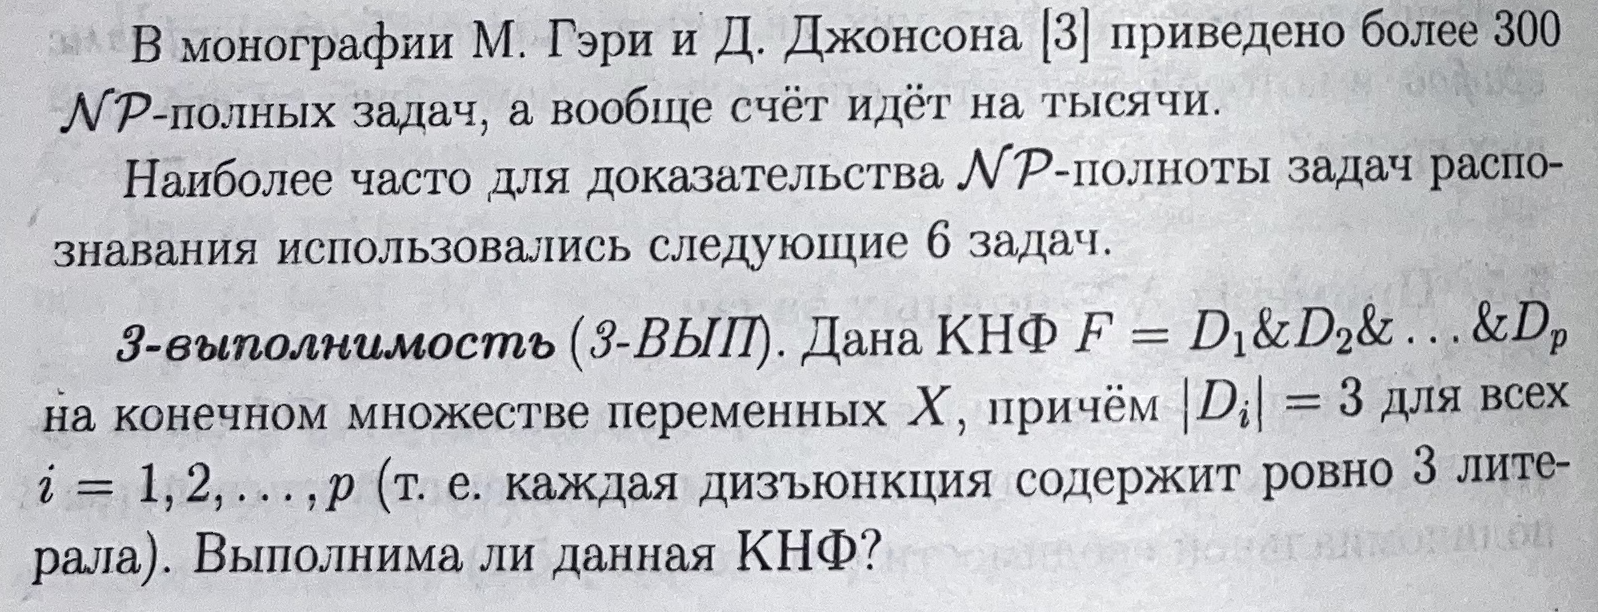
\includegraphics[scale=0.1]{figures/need2.png}
    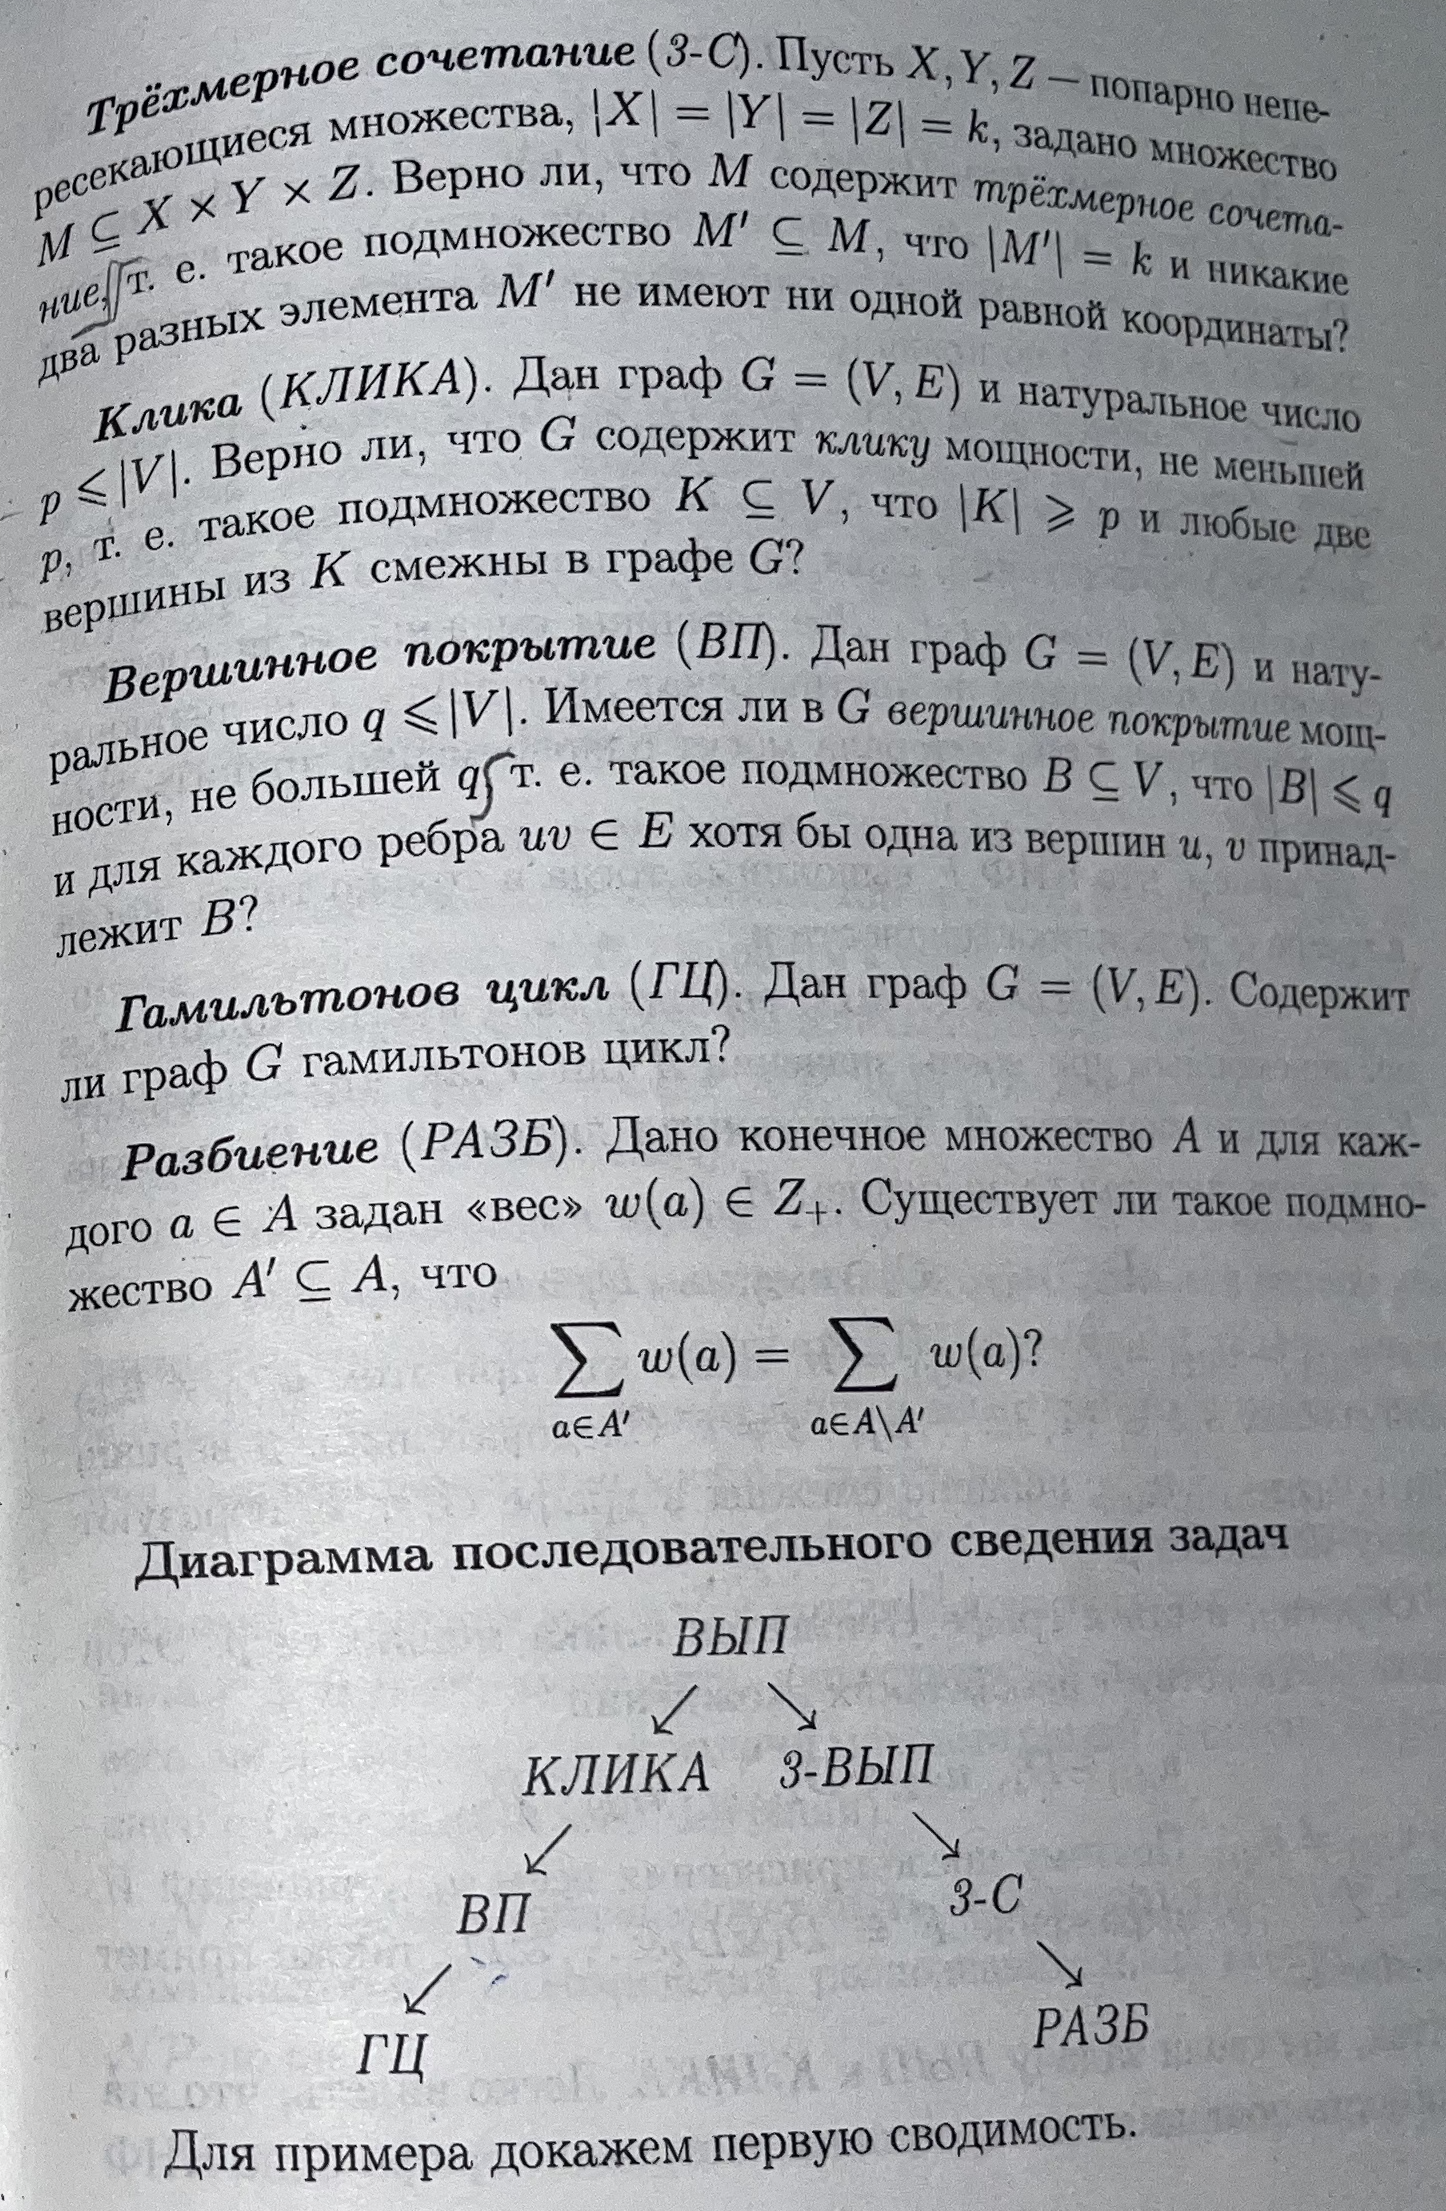
\includegraphics[scale=0.1]{figures/need1.png}
\end{note}
